\documentclass[a4paper,11pt]{article}
\usepackage[a4paper, margin=8em]{geometry}

% usa i pacchetti per la scrittura in italiano
\usepackage[french,italian]{babel}
\usepackage[T1]{fontenc}
\usepackage[utf8]{inputenc}
\frenchspacing 

% usa i pacchetti per la formattazione matematica
\usepackage{amsmath, amssymb, amsthm, amsfonts}

% usa altri pacchetti
\usepackage{gensymb}
\usepackage{hyperref}
\usepackage{standalone}

\usepackage{colortbl}

\usepackage{xstring}
\usepackage{karnaugh-map}

% imposta il titolo
\title{Appunti Sistemi Operativi}
\author{Luca Seggiani}
\date{2025}

% imposta lo stile
% usa helvetica
\usepackage[scaled]{helvet}
% usa palatino
\usepackage{palatino}
% usa un font monospazio guardabile
\usepackage{lmodern}

\renewcommand{\rmdefault}{ppl}
\renewcommand{\sfdefault}{phv}
\renewcommand{\ttdefault}{lmtt}

% circuiti
\usepackage{circuitikz}
\usetikzlibrary{babel}

% testo cerchiato
\newcommand*\circled[1]{\tikz[baseline=(char.base)]{
            \node[shape=circle,draw,inner sep=2pt] (char) {#1};}}

% disponi il titolo
\makeatletter
\renewcommand{\maketitle} {
	\begin{center} 
		\begin{minipage}[t]{.8\textwidth}
			\textsf{\huge\bfseries \@title} 
		\end{minipage}%
		\begin{minipage}[t]{.2\textwidth}
			\raggedleft \vspace{-1.65em}
			\textsf{\small \@author} \vfill
			\textsf{\small \@date}
		\end{minipage}
		\par
	\end{center}

	\thispagestyle{empty}
	\pagestyle{fancy}
}
\makeatother

% disponi teoremi
\usepackage{tcolorbox}
\newtcolorbox[auto counter, number within=section]{theorem}[2][]{%
	colback=blue!10, 
	colframe=blue!40!black, 
	sharp corners=northwest,
	fonttitle=\sffamily\bfseries, 
	title=Teorema~\thetcbcounter: #2, 
	#1
}

% disponi definizioni
\newtcolorbox[auto counter, number within=section]{definition}[2][]{%
	colback=red!10,
	colframe=red!40!black,
	sharp corners=northwest,
	fonttitle=\sffamily\bfseries,
	title=Definizione~\thetcbcounter: #2,
	#1
}

% disponi codice
\usepackage{listings}
\usepackage[table]{xcolor}

\definecolor{codegreen}{rgb}{0,0.6,0}
\definecolor{codegray}{rgb}{0.5,0.5,0.5}
\definecolor{codepurple}{rgb}{0.58,0,0.82}
\definecolor{backcolour}{rgb}{0.95,0.95,0.92}

\lstdefinestyle{codestyle}{
		backgroundcolor=\color{black!5}, 
		commentstyle=\color{codegreen},
		keywordstyle=\bfseries\color{magenta},
		numberstyle=\sffamily\tiny\color{black!60},
		stringstyle=\color{green!50!black},
		basicstyle=\ttfamily\footnotesize,
		breakatwhitespace=false,         
		breaklines=true,                 
		captionpos=b,                    
		keepspaces=true,                 
		numbers=left,                    
		numbersep=5pt,                  
		showspaces=false,                
		showstringspaces=false,
		showtabs=false,                  
		tabsize=2
}

\lstdefinestyle{shellstyle}{
		backgroundcolor=\color{black!5}, 
		basicstyle=\ttfamily\footnotesize\color{black}, 
		commentstyle=\color{black}, 
		keywordstyle=\color{black},
		numberstyle=\color{black!5},
		stringstyle=\color{black}, 
		showspaces=false,
		showstringspaces=false, 
		showtabs=false, 
		tabsize=2, 
		numbers=none, 
		breaklines=true
}


\lstdefinelanguage{assembler}{ 
  keywords={AAA, AAD, AAM, AAS, ADC, ADCB, ADCW, ADCL, ADD, ADDB, ADDW, ADDL, AND, ANDB, ANDW, ANDL,
        ARPL, BOUND, BSF, BSFL, BSFW, BSR, BSRL, BSRW, BSWAP, BT, BTC, BTCB, BTCW, BTCL, BTR, 
        BTRB, BTRW, BTRL, BTS, BTSB, BTSW, BTSL, CALL, CBW, CDQ, CLC, CLD, CLI, CLTS, CMC, CMP,
        CMPB, CMPW, CMPL, CMPS, CMPSB, CMPSD, CMPSW, CMPXCHG, CMPXCHGB, CMPXCHGW, CMPXCHGL,
        CMPXCHG8B, CPUID, CWDE, DAA, DAS, DEC, DECB, DECW, DECL, DIV, DIVB, DIVW, DIVL, ENTER,
        HLT, IDIV, IDIVB, IDIVW, IDIVL, IMUL, IMULB, IMULW, IMULL, IN, INB, INW, INL, INC, INCB,
        INCW, INCL, INS, INSB, INSD, INSW, INT, INT3, INTO, INVD, INVLPG, IRET, IRETD, JA, JAE,
        JB, JBE, JC, JCXZ, JE, JECXZ, JG, JGE, JL, JLE, JMP, JNA, JNAE, JNB, JNBE, JNC, JNE, JNG,
        JNGE, JNL, JNLE, JNO, JNP, JNS, JNZ, JO, JP, JPE, JPO, JS, JZ, LAHF, LAR, LCALL, LDS,
        LEA, LEAVE, LES, LFS, LGDT, LGS, LIDT, LMSW, LOCK, LODSB, LODSD, LODSW, LOOP, LOOPE,
        LOOPNE, LSL, LSS, LTR, MOV, MOVB, MOVW, MOVL, MOVSB, MOVSD, MOVSW, MOVSX, MOVSXB,
        MOVSXW, MOVSXL, MOVZX, MOVZXB, MOVZXW, MOVZXL, MUL, MULB, MULW, MULL, NEG, NEGB, NEGW,
        NEGL, NOP, NOT, NOTB, NOTW, NOTL, OR, ORB, ORW, ORL, OUT, OUTB, OUTW, OUTL, OUTSB, OUTSD,
        OUTSW, POP, POPL, POPW, POPB, POPA, POPAD, POPF, POPFD, PUSH, PUSHL, PUSHW, PUSHB, PUSHA, 
				PUSHAD, PUSHF, PUSHFD, RCL, RCLB, RCLW, MOVSL, MOVSB, MOVSW, STOSL, STOSB, STOSW, LODSB, LODSW,
				LODSL, INSB, INSW, INSL, OUTSB, OUTSL, OUTSW
        RCLL, RCR, RCRB, RCRW, RCRL, RDMSR, RDPMC, RDTSC, REP, REPE, REPNE, RET, ROL, ROLB, ROLW,
        ROLL, ROR, RORB, RORW, RORL, SAHF, SAL, SALB, SALW, SALL, SAR, SARB, SARW, SARL, SBB,
        SBBB, SBBW, SBBL, SCASB, SCASD, SCASW, SETA, SETAE, SETB, SETBE, SETC, SETE, SETG, SETGE,
        SETL, SETLE, SETNA, SETNAE, SETNB, SETNBE, SETNC, SETNE, SETNG, SETNGE, SETNL, SETNLE,
        SETNO, SETNP, SETNS, SETNZ, SETO, SETP, SETPE, SETPO, SETS, SETZ, SGDT, SHL, SHLB, SHLW,
        SHLL, SHLD, SHR, SHRB, SHRW, SHRL, SHRD, SIDT, SLDT, SMSW, STC, STD, STI, STOSB, STOSD,
        STOSW, STR, SUB, SUBB, SUBW, SUBL, TEST, TESTB, TESTW, TESTL, VERR, VERW, WAIT, WBINVD,
        XADD, XADDB, XADDW, XADDL, XCHG, XCHGB, XCHGW, XCHGL, XLAT, XLATB, XOR, XORB, XORW, XORL},
  keywordstyle=\color{blue}\bfseries,
  ndkeywordstyle=\color{darkgray}\bfseries,
  identifierstyle=\color{black},
  sensitive=false,
  comment=[l]{\#},
  morecomment=[s]{/*}{*/},
  commentstyle=\color{purple}\ttfamily,
  stringstyle=\color{red}\ttfamily,
  morestring=[b]',
  morestring=[b]"
}

\lstset{language=assembler, style=codestyle}

% disponi sezioni
\usepackage{titlesec}

\titleformat{\section}
	{\sffamily\Large\bfseries} 
	{\thesection}{1em}{} 
\titleformat{\subsection}
	{\sffamily\large\bfseries}   
	{\thesubsection}{1em}{} 
\titleformat{\subsubsection}
	{\sffamily\normalsize\bfseries} 
	{\thesubsubsection}{1em}{}

% tikz
\usepackage{tikz}

% float
\usepackage{float}

% grafici
\usepackage{pgfplots}
\pgfplotsset{width=10cm,compat=1.9}

% disponi alberi
\usepackage{forest}

\forestset{
	rectstyle/.style={
		for tree={rectangle,draw,font=\large\sffamily}
	},
	roundstyle/.style={
		for tree={circle,draw,font=\large}
	}
}

% disponi algoritmi
\usepackage{algorithm}
\usepackage{algorithmic}
\makeatletter
\renewcommand{\ALG@name}{Algoritmo}
\makeatother

% disponi numeri di pagina
\usepackage{fancyhdr}
\fancyhf{} 
\fancyfoot[L]{\sffamily{\thepage}}

\makeatletter
\fancyhead[L]{\raisebox{1ex}[0pt][0pt]{\sffamily{\@title \ \@date}}} 
\fancyhead[R]{\raisebox{1ex}[0pt][0pt]{\sffamily{\@author}}}
\makeatother

\begin{document}
% sezione (data)
\section{Lezione del 07-10-25}

% stili pagina
\thispagestyle{empty}
\pagestyle{fancy}

% testo
\subsection{Nucleo}
Il \textbf{nucleo} o \textit{kernel} è il cuore di un S/O, il componente che ha il compito di realizzare l'astrazione della \textit{CPU virtuale}. Nel caso di sistemi monoprocessore, vogliamo dividere il tempo fra i processi per dargli l'illusione di essere gli unici in esecuzione sulla macchina.

\subsubsection{Scheduling}
Lo scheduling è l'attività secondo la quale il sistema operativo effettua delle scelte fra quali processi caricare in memoria centrale e a quali assegnare la CPU.

Ci sono 3 diverse attività di scheduling:
\begin{itemize}
	\item \textbf{Breve} termine: lo scheduling propriamente detto, il processo attraverso cui si assegna la CPU. Può essere \textit{preemptive} e \textit{non preemptive} (con o senza diritto di revoca). Solitamente viene invocato molto frequentemente (millisecondi);
	\item \textbf{Medio} termine (\textit{swapping}): il trasferimento temporaneo in memoria secondaria dei processi. Si usa quando la memoria centrale dispone di memoria minore della somma di quella richiesta dai vari processi. Viene invocato più di rado (secondi, minuti);
	\item \textbf{Lungo} termine: la scelta di quali processi caricare dalla memoria secondaria in memoria centrale. Rappresenta un componente importante dei sistemi \textit{batch} multiprogrammati, oggi come oggi quindi sui \textit{server} e meno sulle macchine personali;
\end{itemize}

Vediamo quindi una schematica che mostra dove queste attività di scheduling avvengono nell'architettura vista:
\begin{center}
	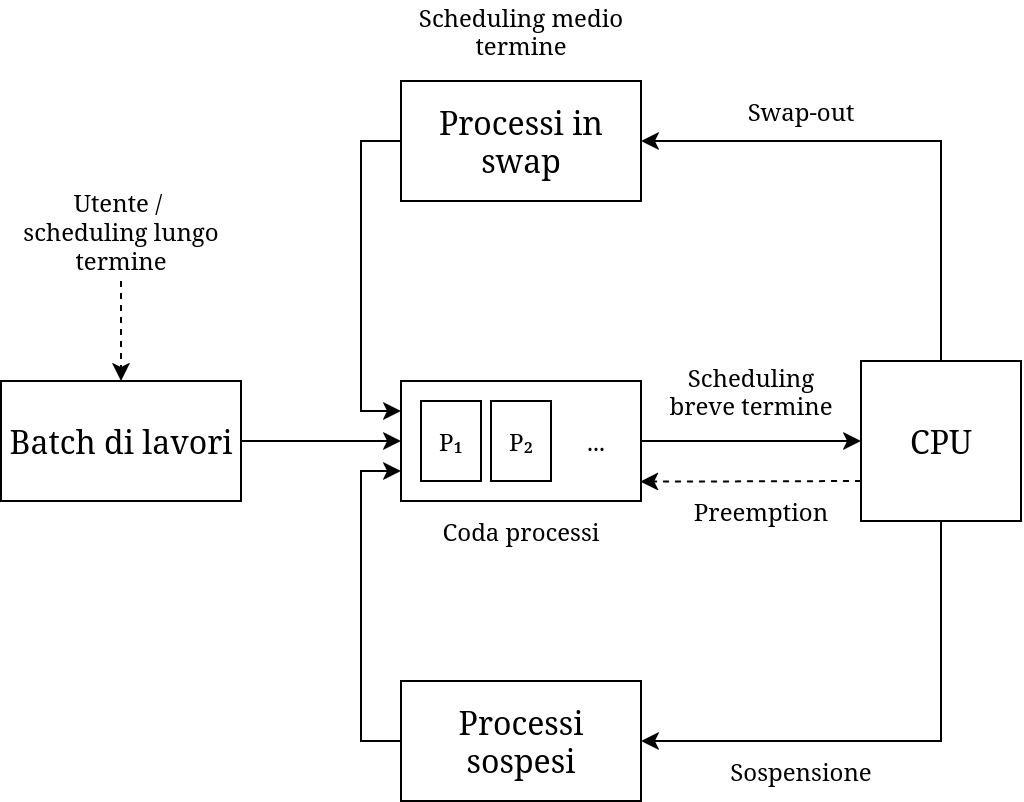
\includegraphics[scale=0.3]{../figures/scheduling.png}
\end{center}

I processi possono in genere classificarsi in:
\begin{itemize}
	\item Processi vincolati da \textbf{I/O}: passano più tempo a fare I/O burst piuttosto che CPU burst (che sono tanti e piccoli);
	\item Processi vincolati da \textbf{CPU}: passano più tempo a fare calcoli, hanno pochi e lunghi CPU burst.
\end{itemize}

\subsection{Algoritmi di scheduling}
Gli algoritmi di scheduling che vedremo saranno:
\begin{itemize}
	\item \textbf{FCFS} (\textit{First Come First Served}): è \textit{non prioritario} e \textit{non preemptive}, consiste nel assegnare la CPU sempre al primo processo arrivato;
	\item \textbf{SJF} (\textit{Shortest Job First}): è \textit{prioritario} e \textit{non preemptive}, consiste nell'assegnare la CPU al processo più breve;
	\item \textbf{SRTF} (\textit{Shortest Remaining Time First}): è \textit{prioritario} e \textit{preemptive}, rappresenta sostanzialmente la versione con revoca del precedente;
	\item \textbf{RR} (\textit{Round Robin}): è \textit{non prioritario} e \textit{preemptive}: si basa sull'assegnare quanti temporali ugualmente ad ogni processo;
	\item Schedulazione \textbf{su base prioritaria}: introdurremo qui l'idea di \textit{priorità} per ogni processo;
	\item Schedulazione \textbf{a code multiple}: prevediamo più code, che possiamo distinguere usando gli algoritmi sopra descritti, o come vedremo sarà conveniente, assegnando una \textit{priorità} ad ogni cosa;
	\item Schedulazione di sistemi \textbf{in tempo reale}. Questi sono algoritmi che devono assicurare la terminazione deterministicad ei processi. In questo vedremo gli algoritmi:
		\begin{itemize}
			\item \textbf{RM} (\textit{Rate Monotonic});
			\item \textbf{EDF} (\textit{Earliest Deadline First}).
		\end{itemize}
\end{itemize}

\subsubsection{Valutazione degli algoritmi di scheduling}
Iniziamo a vedere alcune metriche per la valutazione degli algoritmi di scheduling:

\begin{center}
	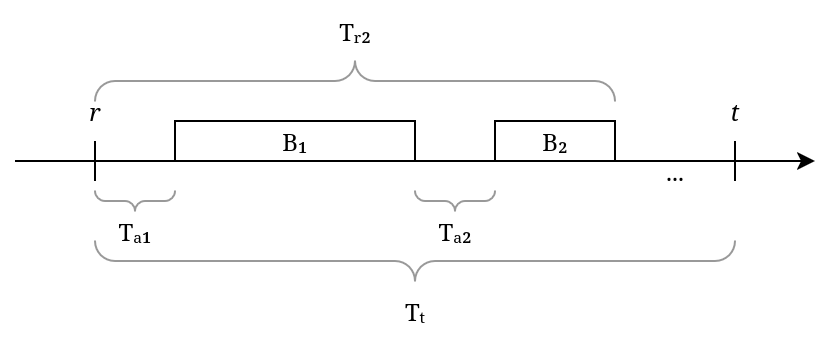
\includegraphics[scale=0.4]{../figures/scheduling_valuta.png}
\end{center}

\begin{itemize}
	\item \textbf{Utilizzazione} della CPU o \textit{efficienza}, cioè definito $\Delta B_i$ il tempo di burst e $T$ il quanto di tempo totale, vogliamo un efficienza $E$:
		$$
			E = \frac{\sum \Delta B_i}{T} < 1
		$$
		il più possibile vicina a 1;
	\item Tempo medio di \textbf{completamento} (o tempo di \textit{turnaround}), cioè il tempo che passa prima che il processo possa completare la sua operazione (terminando). Prendiamo l'istante in cui il processo entra in coda pronti come $r$ (da \textit{richiesto}) e quello in cui termina termina come $t$ (da \textit{termina}). Il tempo di completamento $T_t$ sarà ovviamente:
		$$
			T_t = t - r
		$$
	\item \textbf{Produttività} (o frequenza di \textit{througput}), definita come il numero medio di processi completati nell'unità di tempo, cioè l'inverso del tempo medio di completamento:
		$$
			P = \frac{1}{T_t}
		$$
	\item Tempo di \textbf{risposta}, valutato dall'istante in cui un processo entra in coda pronti $r$ all'istante in cui risponde, cioè termina un CPU burst (solitamente il primo). Purtroppo, non tutto il tempo di completamento $T_c$ è dedicato al processo, ma questo viene eseguito, come sappiamo, in più burst (diciamo $B_1$, $B_2$, ...). Il tempo di turnaround $T_t$ sarà allora il tempo trascorso fra $r$ e la fine di un burst $B_i$, cioè:
		$$
			{T_r}_i = \text{end}(B_i) - r
		$$
	\item Tempo di \textbf{attesa}, cioè la somma dei tempi di attesa posti fra i vari burst:
		$$
		T_a = \sum {t_\alpha}_i
		$$
		Con riferimento ai sistemi interattivi, spesso ci interessa il tempo di attesa iniziale, cioè quello fra l'inserimento in coda pronti e l'inizio del primo CPU burst, o in relazione al nostro schema:
		$$
		T_a' = {t_\alpha}_1 = r - \text{begin}(B_1)
		$$

		Dovrebbe essere chiaro che il tempo di \textit{attesa} si distingue dal tempo di \textit{risposta}, in quanto:
		\begin{itemize}
			\item Il tempo di attesa è quello visto dal \textit{processo} prima che questo possa iniziare la computazione;
			\item Il tempo di risposta è quello visto dall'\textit{utente} prima di vedersi tornare un primo risultato (si presume che alla fine dei CPU burst inizia un I/O burst che porta avanti qualche operazione di lettura o scritture da periferiche, tangibile per l'utente).
		\end{itemize}
	\item Rispetto dei \textbf{vincoli temporali}, utile principalmente negli algoritmi di scheduling in \textit{tempo reale}.
\end{itemize}

Fra queste metriche, tempo di \textbf{risposta} e di \textbf{attesa} sono relativi principalmente ai \textit{sistemi interattivi}, mentre il rispetto dei \textbf{vincoli temporali} è relativo ai sistemi in \textit{tempo reale}.

Chiameremo poi $O_v$ l'\textbf{overhead} associato all'esecuzione dello scheduler. Ricordiamo che in ogni caso in questa fase stiamo parlando di scheduling a breve termine.

\subsubsection{Algoritmo FCFS}
Nell'algoritmo \textbf{FCFS} (\textit{First Come First Served}) assegnamo la CPU al primo processo in coda pronti. Sostanzialmente, trattiamo la coda pronti come una coda \textbf{FIFO} (\textit{First In, First Out}).
Questo lo rende non prioritario e non preemptive.

Quello che otteniamo è un efficienza teorica pari a $E\sim1$ (c'è un piccolo overhead $O_v \sim 0$ dato dal cambio di contesto), ma generalmente prestazioni piuttosto limitate.
Questo è dovuto al fatto che i tempi di attesa (e di conseguenza di completamento) dei processi sono completamente aleatori, e non si fa alcuna scelta informata mirata a minimizzarli.

%\par\smallskip
\newpage

Vediamo ad esempio il comportamento ottenuto con la sequenza di processi:
\begin{table}[H]
	\center \rowcolors{2}{white}{black!10}
	\begin{tabular} { c || c | c }
		\bfseries Processo & \bfseries $\mathbf{T}$ richiesta & \bfseries $\mathbf{C}$ esecuzione \\
		\hline
		$p_0$ & 0 & 10 \\ 
		$p_1$ & 2 & 100 \\ 
		$p_2$ & 4 & 24 \\ 
		$p_3$ & 6 & 16 
	\end{tabular}
\end{table}

Su un grafico con il tempo $t$ alle ascisse, avremo:
\begin{center}
	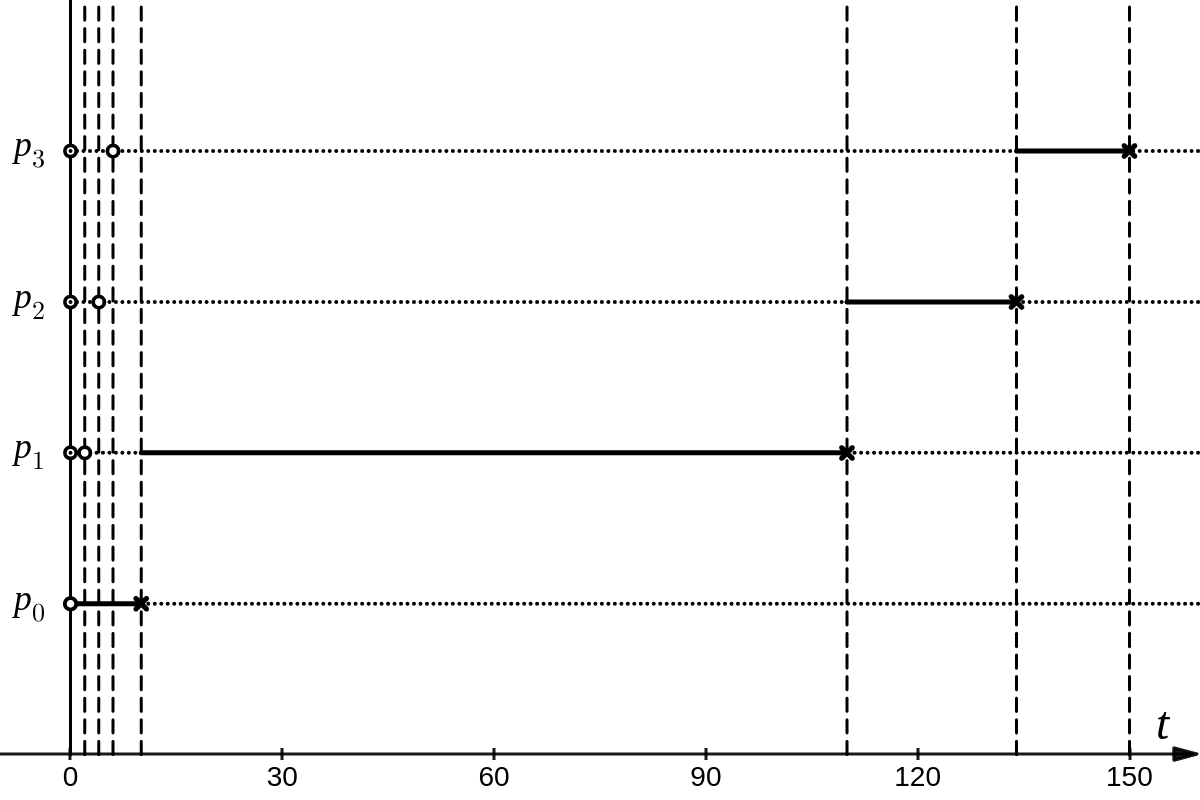
\includegraphics[scale=0.3]{../figures/fcfs_bad.png}
\end{center}

Questo risulta in un tempo medio di attesa di:
$$
\tilde{t}_a = \frac{{t_a}_0 + {t_a}_1 + {t_a}_2 + {t_a}_3}{4} = \frac{0 + 8 + 106 + 128}{4} = 60.5
$$

Vediamo come questo comportamento può cambiare radicalmente cambiando l'ordine di richiesta dei processi. Poniamo infatti di avere la sequenza:
\begin{table}[H]
	\center \rowcolors{2}{white}{black!10}
	\begin{tabular} { c || c | c }
		\bfseries Processo & \bfseries $\mathbf{T}$ richiesta & \bfseries $\mathbf{C}$ esecuzione \\
		\hline
		$p_0$ & 0 & 10 \\ 
		$p_1$ & 6 & 100 \\ 
		$p_2$ & 4 & 24 \\ 
		$p_3$ & 2 & 16 
	\end{tabular}
\end{table}
dove semplicemente si è invertito l'ordine degli ultimi 3 processi. 

\newpage

Sul grafico avremo:
\begin{center}
	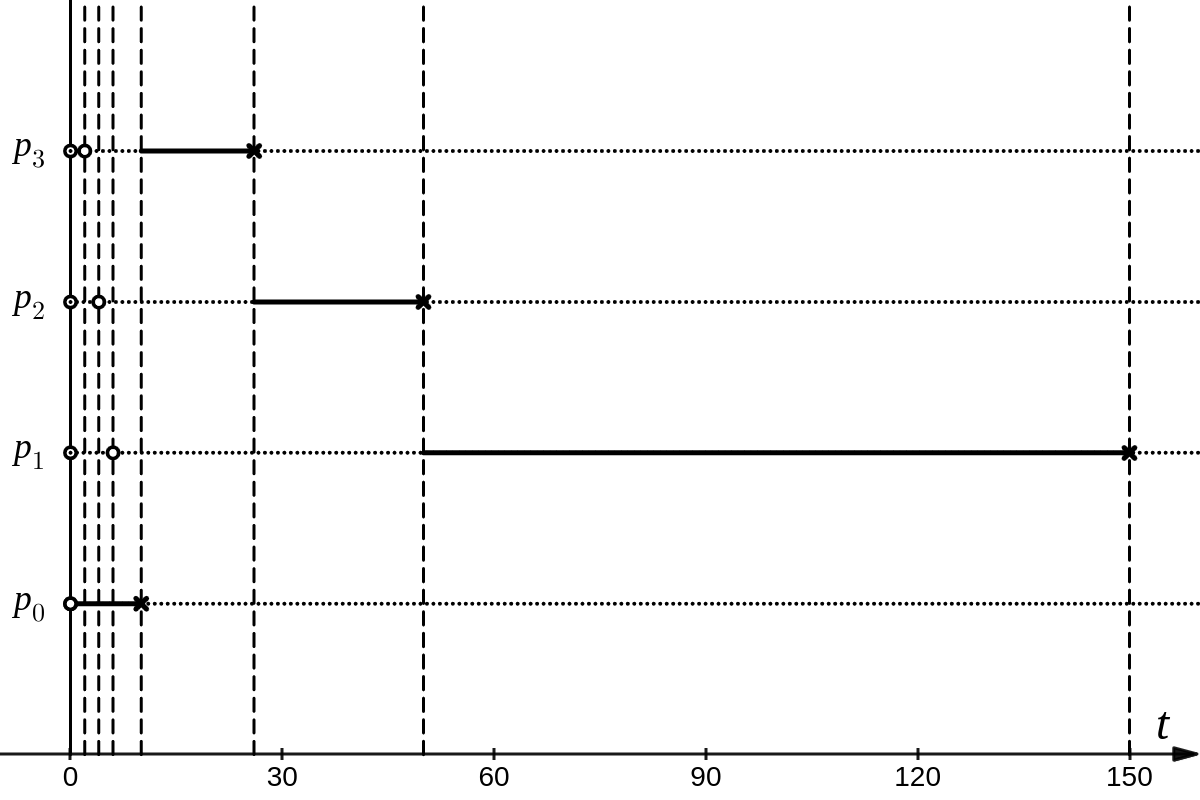
\includegraphics[scale=0.3]{../figures/fcfs_good.png}
\end{center}

Questo risulta in un tempo medio di attesa di:
$$
\tilde{t}_a = \frac{{t_a}_0 + {t_a}_1 + {t_a}_2 + {t_a}_3}{4} = \frac{0 + 44 + 22 + 8}{4} = 18.5
$$
Chiaramente molto meglio del caso precedente.

\par\smallskip

Abbiamo quindi che l'algoritmo è utile per sistemi batch, dove l'unica cosa che ci interessa è uso massimo della CPU (che ci assicura), ma largamente da evitare per sistemi interattivi, e sopratutto per sistemi real-time.
Questo è vouto all'aleatorietà legata al momento della richiesta dei processi, che rende impossibile rispondere celeremente o fare qualsiasi tipo di promessa sul tempo di turnaround.

\subsubsection{Algoritmo SJF}
L'algoritmo \textbf{SJF} (\textit{Shortest Job First}) implementa una \textbf{priorità statica}: si fa l'ipotesi di conoscere il \textbf{tempo di CPU} utilizzato da ogni processo, e assegnare priorità maggiori a processi con tempo di esecuzione minore. Di contro, non è preemptive, cioè una volta assegnata la CPU non può revocarla. Su come il S/O conosce il tempo di esecuzione non facciamo per adesso ipotesi. 

\par\smallskip

Simuliamo anche questo algoritmo, usando la stessa tabella del primo caso in 6.2.2:
\begin{table}[H]
	\center \rowcolors{2}{white}{black!10}
	\begin{tabular} { c || c | c }
		\bfseries Processo & \bfseries $\mathbf{T}$ richiesta & \bfseries $\mathbf{C}$ esecuzione \\
		\hline
		$p_0$ & 0 & 10 \\ 
		$p_1$ & 2 & 100 \\ 
		$p_2$ & 4 & 24 \\ 
		$p_3$ & 6 & 16 
	\end{tabular}
\end{table}

\newpage

Osserviamo che applicando l'algoritmo si ottiene il flusso di esecuzione:
\begin{center}
	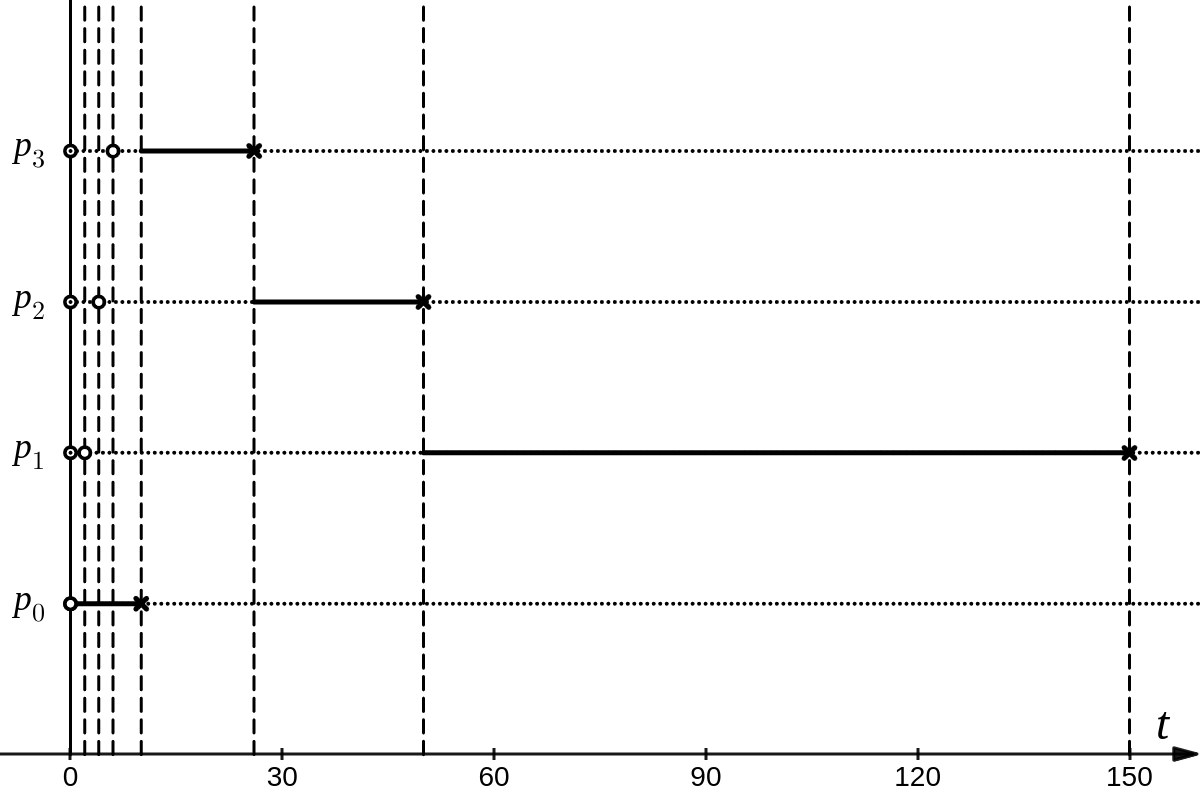
\includegraphics[scale=0.3]{../figures/sjf.png}
\end{center}
Cioè esattamente quello che avevamo visto come caso ottimo del FCFS (che ricordiamo aveva tempo medio $\tilde{T}_a = 18.5$), senza che i processi siano arrivati necessariamente nell'ordine ottimo.

\par\smallskip

Facciamo una nota sulla priorità statica: ad ogni chiamata dello scheduler questo può sapere solo i tempi di esecuzione dei processi attualmente in esecuzione, cioè si potrebbe mandare in esecuzione un processo con tempo di esecuzione maggiore quando ne entra in coda pronti ne entra uno con tempo minore. 
In questo caso, per la natura \textit{non preemptive} dell'algoritmo, bisogna lasciare che questo esegua prima di mettere il nuovo arrivato in esecuzione.

Adoperando questo algoritmo si minimizza (nel senso matematicamente ottimo) il tempo di attesa medio dei processi, in quanto si cerca di arrivare il prima possibile al processo sucessivo (svolgendo adesso il più veloce).
Uno svantaggio sarà chiaramente che i processi che dimostrano tempi di esecuzione lunghi verranno eseguiti sempre per ultimi.

\subsubsection{Algoritmo SRTF}
Abbiamo introdotto l'algoritmo \textbf{SRTF} (\textit{Shortest Remaining Time First}) come una versione \textit{preemptive} del SJF (in questo rimane comunque prioritario).

Visto che è preemptive, viene eseguito \textit{ogni volta} che cambiano le condizioni di scelta (non soltanto quando la CPU è libera, come nel caso dei non preemptive, ma ogni che un nuovo processo entra in esecuzione).
Può per questo motivo eseguire senza innescare cambi di contesto.

Dovremmo adattare la nostra ipotesi di conoscenza del tempo di CPU ad un'ipotesi di conoscenza del \textbf{tempo rimanente} per ogni processo: in questo caso se il processo appena entrato ha tempo rimanente minore di quello del processo attualmente in esecuzione, conviene sfruttare la preemption.
Di nuovo, per adesso non facciamo assunzioni su come ricaviamo tale euristica.

L'unica considerazione che ci conviene fare è che aggiornare le previsioni temporali ad ogni evento che cambia le condizioni di scelta chiede allo scheduler di fare più conti, e quindi aumenta leggermente l'overhead $O_v$.
Ampia letteratura dimostra che l'approccio è comunque conveniente. 

\par\smallskip

Simuliamo questo algoritmo con la tabella, modificata dalle precedenti mandando per primo in esecuzione il processo $p_1$, con tempo di esecuzione maggiore:
\begin{table}[H]
	\center \rowcolors{2}{white}{black!10}
	\begin{tabular} { c || c | c }
		\bfseries Processo & \bfseries $\mathbf{T}$ richiesta & \bfseries $\mathbf{C}$ esecuzione \\
		\hline
		$p_0$ & 2 & 10 \\ 
		$p_1$ & 0 & 100 \\ 
		$p_2$ & 4 & 24 \\ 
		$p_3$ & 6 & 16 
	\end{tabular}
\end{table}

Osserviamo che applicando l'algoritmo si ottiene il flusso di esecuzione:
\begin{center}
	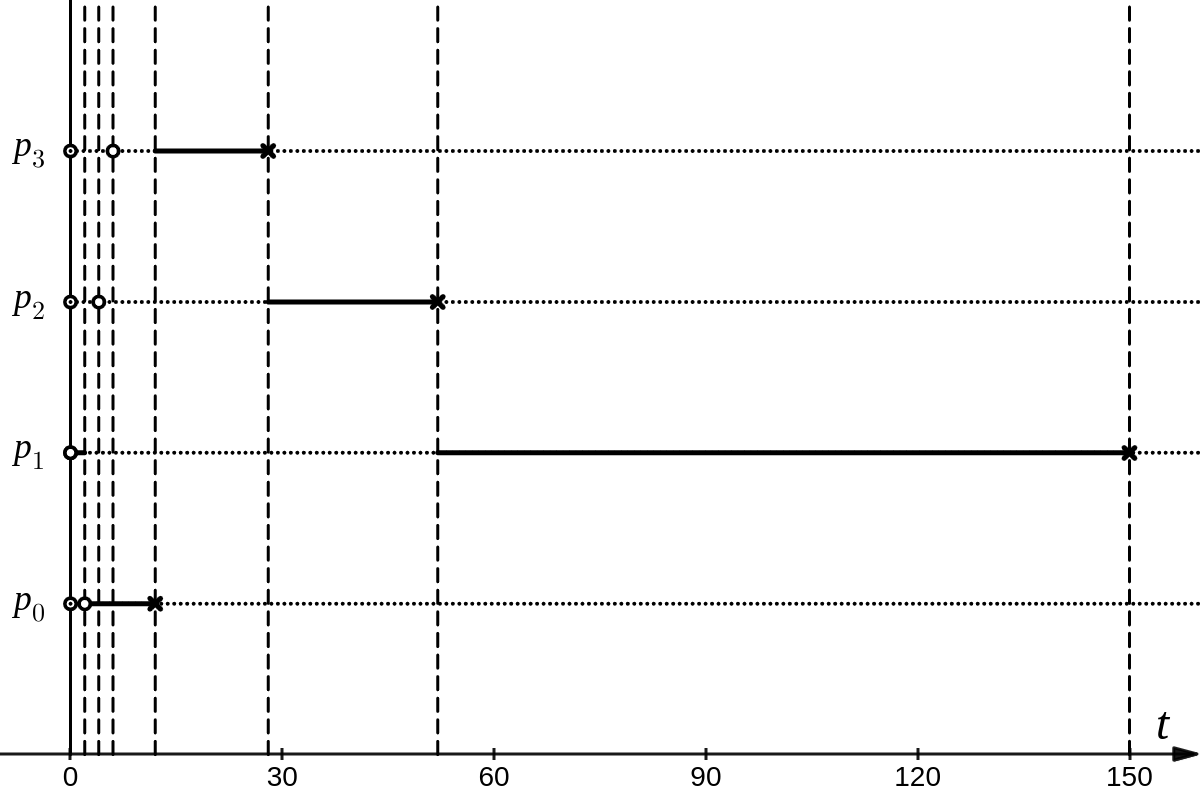
\includegraphics[scale=0.3]{../figures/srtf.png}
\end{center}

Questo risulta in un tempo medio di attesa di:
$$
\tilde{t}_a = \frac{{t_a}_0 + {t_a}_1 + {t_a}_2 + {t_a}_3}{4} = \frac{2 + 0 + 28 + 12}{4} = 10.5
$$
prima del primo burst.

Ciò che è importante in questo caso è che il processo $p_1$ viene sospeso con preemption per permettere l'esecuzione dei CPU burst di $p_0$, $p_2$ e $p_3$, molto più veloci. In questo modo il sistema risulta nel complesso molto più responsivo.

\par\smallskip

L'SRTF migliora la risposta in tempo reale del SJF, permettendo una riduzione sia dei tempi di turnaround che dei tempi di attesa medi in caso di richieste di esecuzione di processi non ottimali. 

Un problema del SRTF, come avevamo visto nel SJF, e la \textbf{process starvation}: in genere, negli algoritmi in base prioritaria, si rischia che i processi a priorità minore (in questo caso quelli con tempo rimanente maggiore) non vengano mai serviti e rimangano a lungo in coda pronti, rendendo il sistema meno responsivo.

Anche qui la letteratura ci rende noto che la priorità dei processi in SRTF è \textbf{monotona crescente}: man di mano che i processi eseguono, il loro tempo rimanente diminuisce e quindi la priorità aumenta. Questo effetto aiuta a ridurre la process starvation.

\subsubsection{Stima dei tempi in SJF e SRTF}
Chiariamo la questione di come si possono fare previsioni informate sul \textbf{tempo di esecuzione} (in \textit{SJF}) e il \textbf{tempo rimanente} (in \textit{SRTF}).

Un'approccio, preso ad esempio il caso del \textbf{tempo di esecuzione}, è quello di usare la tecnica della \textbf{esponenziale}.
Si fa una stima iniziale $s_i$ del tempo di burst $t_i$ esimo.
Preso un parametro $a$ con $0 < a < 1$, si aggiorna ad ogni terminazione del processo (quindi facendo delle \textit{osservazioni} per ogni esecuzione del processo) la stima come:
$$
s_{n + 1} = a t_n + (1 - a) s_n
$$

Presi $a \sim 0$ si ha che le stime deviano malvolentieri da quella iniziale, mentre con $a \sim 1$ si ha che le stime sono molto volubili rispetto alle osservazioni fatte. 

Modeli statistici più complessi possono dare previsioni più accurate, sempre tenendo conto del fatto che lo scheduler deve eseguire con overhead $O_v \sim 0$, o almeno il più piccolo possibile.

Una volta noto il \textit{tempo di esecuzione}, il \textbf{tempo rimanente} si può stimare considerando il tempo che il processo ha impiegato finora e sottraendolo dal tempo di esecuzione totale (se non rinunciando al tener conto se tale tempo è stato usato in CPU o I/O burst, purtroppo un'euristica è un'euristica).

\end{document}
